\documentclass[11pt, oneside]{article}   	% use "amsart" instead of "article" for AMSLaTeX format
\usepackage{geometry}                		% See geometry.pdf to learn the layout options. There are lots.
\geometry{letterpaper}                   		% ... or a4paper or a5paper or ... 
%\geometry{landscape}                		% Activate for rotated page geometry
%\usepackage[parfill]{parskip}    		% Activate to begin paragraphs with an empty line rather than an indent
\usepackage{graphicx}				% Use pdf, png, jpg, or eps§ with pdflatex; use eps in DVI mode
								% TeX will automatically convert eps --> pdf in pdflatex		
\usepackage{amssymb}

%SetFonts

%SetFonts
\setlength{\parindent}{0pt}

\title{Lecture Note 7 }
\author{Yiping Lu, Jody Shu and Jashaina Thomas}

%\date{}							% Activate to display a given date or no date

\begin{document}
\begin{Large}
\maketitle
\section{Softmax Regression Algorithm}
%\subsection{}

Softmax is an extension of Logistic Regression (LR).

LR setup : $y \in \{0,1\} \leftarrow discrete$\\
want: $h_\theta \in [0,1]$
\begin{figure}[h] %  figure placement: here, top, bottom, or page
   \centering
   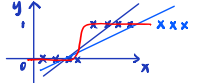
\includegraphics[width=3in]{logisticRegressionPlot} 
\end{figure}
\\
Linear reg: [ -$\infty, \infty$ ]\\
Choose:  $h_\theta (x)=g(\theta^T x)= \frac{1}{1+e^{-\theta^Tx}}$ ,
\\
where $g(z)=\frac{1}{1+e^{-z}}$
\\ (note: $z\rightarrow -\infty \ g(z), \rightarrow 0$,\\
            $\hspace{30pt} z\rightarrow \infty \ g(z), \rightarrow 1)$\\
g is called sigmoid/Logistic function\\
Here: g:$(-\infty, \infty) \rightarrow (0,1)$

p(y=1$\mid x; \theta)=h_\theta (x)=\frac{1}{1+e^{-\theta ^T x}}$\\
p(y=0$\mid y; \theta)=1-h_\theta (x) \geq 0 \ (0 \leq h_\theta (x) \leq 1)$
\\
Next, we are going to write the prob. fcn into one equation.










\end{Large}
\end{document}